% # Ontwerp
% ## ...
% ##


\subsection{De oplaadbare voeding van het systeem} \label{sec:energy}

De sensormodule heeft energie nodig om te functioneren. Deze energie moet geleverd worden door een energie management systeem in de vorm van een constante spanning. Het voedingsblok ligt buiten het signaalverwerkingspad, zoals te zien is in \cref{fig:moduleDiagram_energie}.

\begin{figure}[!htbp]
    \centering
    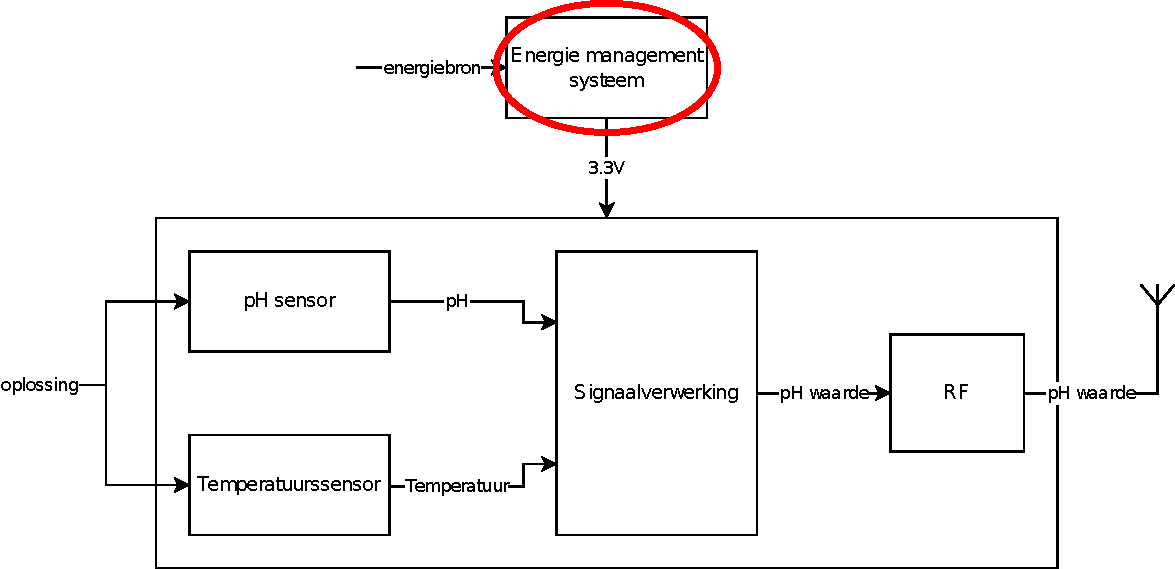
\includegraphics[width=.7\textwidth]{moduleDiagram_energie}
    \caption{De locatie van het energie management systeem in het blokschema van de sensormodule.}
    \label{fig:moduleDiagram_energie}
\end{figure}

Het energie management systeem moet energie kunnen opnemen uit de omgeving, en dit kunnen opslaan. Hiervoor zijn een energy harvesting systeem en een accu nodig.

\subsubsection{Energy Harvesting} \label{sec:harvesting}

Vanuit de opdrachtdefinitie is er gekozen voor een piëzo element. Deze piëzo kan mechanische trillingen omzetten naar elektrische energie. Deze energie kan gebruikt worden om de accu op te laden of het vermogensverbruik van de module te verminderen.

Een piëzo element produceert energie in de vorm van wisselspanning. Deze spanningen kunnen oplopen tot spanningen boven de \qty{20}{\volt}.% TODO: bron????
Hierdoor zal er, naast een gelijkrichter en een spanningsregelaar, ook een beveiliging tussen het piëzo element en de rest van het systeem geplaatst moeten worden.


\subsubsection{Accu} \label{sec:batterijOntwerp}
Er zijn veel verschillende soorten soorten oplaadbare batterijen die gebruikt kunnen worden bij een sensor module. 
Voor de type sensor module waar dit verslag over gaat is gekeken naar 4 verschillende oplaadbare accu opties\cite{battery_comparison}:

\begin{enumerate}
    \item Lithium-Ion (Li-Ion)
    \item Lithium Polymeer (Li-Po)
    \item Zebra (Zout nickel) 
    \item Nickel-Cadmium (Ni-Cd)
\end{enumerate}

In onderzoek \cite{battery_comparison} is het duidelijk aangetoond dat Li-Po het hoogste energiedichtheid heeft. Dit zou een praktische overweging zijn om de sensor module compact te houden. Dit heeft ervoor gezorgd dat voor de sensor module ontwerp een LiPo gekozen is als batterij. Spanning van een cel (1s) LiPo is maximaal 4.2 V en minimaal veilige spanning is 2.7 V\cite{BatteryComparison}. Dit is een van de specificaties van de batterij management systeem. 


\subsubsection{Voeding} \label{sec:voeding}
De voedingsspanning is gekozen vanuit de maximale spanning die nodig is voor de ISFET sensor\cite{isfet}. Hieruit volgt een maximale systeemspanning van \qty{3.3}{\volt}.

Zoals te lezen in \cref{sec:batterijOntwerp} is er gekozen voor LiPo batterij technologie. De batterij heeft een beveiliging voor beide op- en ontladen nodig. De celspanning moet omgezet worden naar systeemspanning van \qty{3.3}{\volt}. Dit kan op meerdere manieren gedaan worden. Twee hiervan zijn een DC-DC buck-boost converter en een low dropout regelaar (LDO). De buck-boost converter is efficiënter dan de LDO, maar heeft een minder stabiele uitgang. Hierdoor is ervoor gekozen om beide soorten regelaar te gebruiken. Dit is te zien in \cref{fig:voedingSchematisch}. Het digitale gedeelte van het systeem wordt gevoed door een buck-boost converter; de spanningsrimpel van de buck-boost converter maakt minder uit voor een goed ontkoppelde microcontroller.
De uitgang van de buck-boost converter wordt vervolgens gestabiliseerd door een LDO, die het analoge gedeelte van het systeem voedt. De uitgangsspanning van de LDO zal iets lager zijn dan de uitgang van de buck-boost converter, wat geen problemen zal vormen zolang het verschil minimaal is.

Zoals beschreven in \cref{sec:harvesting} moet de uitgang van het piëzo element gelijk gericht en beschermt worden. In \cref{fig:voedingSchematisch} wordt het gelijkrichten gedaan door de AC-DC omvormer.

Voor energy harvesting is er een piëzo element gekozen. Een piëzo element kan gezien worden als een AC bron. Deze AC bron moet omgezet worden naar DC die door het systeem gebruikt kan worden om de batterij mee op te laden. De AC bron wordt met een gelijkrichter naar DC omgezet. Deze DC spanning is niet hetzelfde als de systeemspanning dus die moet omgezet worden naar een spanning die de batterij in gaat, zodat de batterij kan opladen.

\begin{figure}[!htbp]
    \centering
    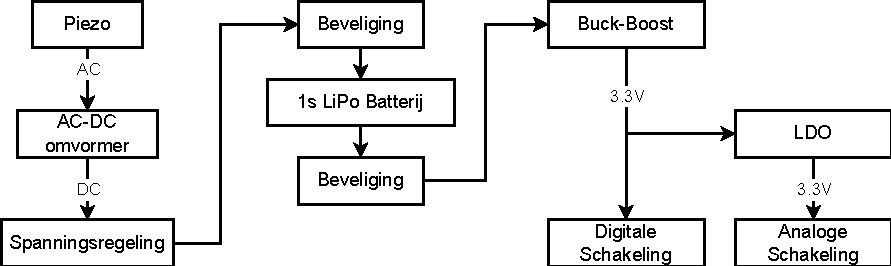
\includegraphics{voedingSchematisch.pdf}
    \caption{Voeding schematisch}
    \label{fig:voedingSchematisch}
\end{figure}



\subsubsection{Energie budget}\label{sec:energyBudgets}
Voor het energiebudget zijn de waardes in \cref{tab:energieBudgetEstimatie} gekozen. Elk van deze waardes ligt boven het theoretisch berekende minimum van het respectievelijke systeemonderdeel. De som van de vermogens is \qty{9}{\milli\watt}, wat onder het maximale toegestane vermogensverbruik van \qty{10}{\milli\watt} ligt.


\begin{table}[!htbp]
    \centering
    \begin{tabular}{l|l}
        Func. blok          & Vermogen [mW] \\
        \hline
        Reken $U_{GS}\rightarrow$pH & 0.6   \\
        ADC                 & 1             \\
        AA-filter           & 0.2           \\
        Meet $U_{GS}$       & 0.2           \\
        Zenden              & 5             \\
        Oplader             & 0.5           \\
        Beveiliging         & 0.5           \\
        Spanningsregeling   & 1             \\
        \hline
        \hline
        Totaal              & 9

    \end{tabular}
    \caption{Energie budget}
    \label{tab:energieBudgetEstimatie}
\end{table}


